% ==========================================================
\section{TikZ Graphics (TikZ 绘图)}
% ==========================================================

\subsection{Basic Geometries (基本几何)}

\subsubsection{功能介绍 (Introduction)} 

TikZ 是 LaTeX 中最强大的绘图工具。一切从基本几何图形开始。

TikZ is the most powerful drawing tool in LaTeX. It all starts with basic geometric shapes.

\vspace{0.5em}
\subsubsection{代码展示 (Code)}

\begin{lstlisting}[language=TeX]
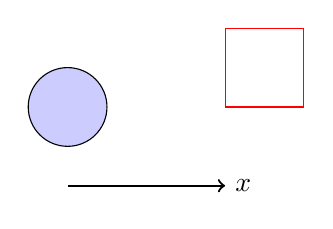
\begin{tikzpicture}
    \draw[thick, ->] (0,0) -- (2,0) node[right] {$x$};
    \draw[fill=blue!20] (0,1) circle (0.5);
    \draw[red] (2,1) rectangle (3,2);
\end{tikzpicture}
\end{lstlisting}

\subsubsection{语法详解 (Syntax)}

\begin{itemize}
    \item \code{\textbackslash draw}: 绘制路径。
    \item \code{(x,y)}: 笛卡尔坐标。
    \item \code{--}: 直线连接。
    \item \code{circle (radius)}: 圆。
    \item \code{rectangle (corner)}: 矩形。
\end{itemize}

\subsubsection{效果展示 (Effect)}

\begin{center}
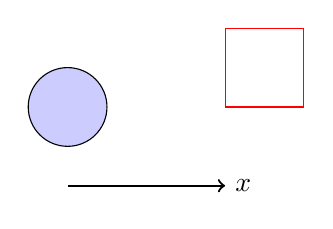
\begin{tikzpicture}
    \draw[thick, ->] (0,0) -- (2,0) node[right] {$x$};
    \draw[fill=blue!20] (0,1) circle (0.5);
    \draw[red] (2,1) rectangle (3,2);
\end{tikzpicture}
\end{center}

\subsection{Flowcharts (流程图)}

\subsubsection{功能介绍 (Introduction)} 

利用 \texttt{otex.sty} 中预定义的样式快速绘制流程图。

Quickly draw flowcharts using predefined styles in \texttt{otex.sty}.

\vspace{0.5em}
\subsubsection{代码展示 (Code)}

\begin{lstlisting}[language=TeX]
\begin{tikzpicture}[node distance=1.5cm]
    \node (start) [startstop] {Start};
    \node (pro1) [process, below of=start] {Process};
    \node (dec1) [decision, below of=pro1] {Check?};
    \draw [arrow] (start) -- (pro1);
    \draw [arrow] (pro1) -- (dec1);
\end{tikzpicture}
\end{lstlisting}

\subsubsection{语法详解 (Syntax)}

\begin{itemize}
    \item \code{\textbackslash node (name) [style] \{text\}}: 定义节点。
    \item \code{below of=node}: 相对定位 (需 \texttt{positioning} 库)。
    \item \code{startstop}, \code{process}, \code{decision}: 预定义样式。
\end{itemize}

\subsubsection{效果展示 (Effect)}

\begin{center}
\begin{tikzpicture}[node distance=1.5cm]
    \node (start) [startstop] {Start};
    \node (pro1) [process, below of=start] {Process};
    \node (dec1) [decision, below of=pro1] {Check?};
    \draw [arrow] (start) -- (pro1);
    \draw [arrow] (pro1) -- (dec1);
\end{tikzpicture}
\end{center}

\subsection{Tree Diagrams (树形图)}

\subsubsection{功能介绍 (Introduction)} 

TikZ 的 \texttt{child} 语法使得绘制树形结构变得非常直观。

TikZ's \texttt{child} syntax makes drawing tree structures very intuitive.

\vspace{0.5em}
\subsubsection{代码展示 (Code)}

\begin{lstlisting}[language=TeX]
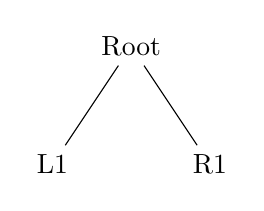
\begin{tikzpicture}[level 1/.style={sibling distance=2cm}]
    \node {Root}
        child { node {L1} }
        child { node {R1} };
\end{tikzpicture}
\end{lstlisting}

\subsubsection{语法详解 (Syntax)}

\begin{itemize}
    \item \code{child \{ node \{...\} \}}: 定义子节点。
    \item \code{sibling distance}: 设置兄弟节点间距。
\end{itemize}

\subsubsection{效果展示 (Effect)}

\begin{center}
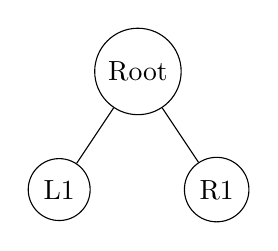
\begin{tikzpicture}[level 1/.style={sibling distance=2cm}, every node/.style={circle,draw}]
    \node {Root}
        child { node {L1} }
        child { node {R1} };
\end{tikzpicture}
\end{center}
